% ---- Chicago Thesis Style ---- %
%\documentclass[truedoublespace]{ccw_chithesis}
\documentclass[singlespace]{ccw_chithesis}
\usepackage{url}
\usepackage{graphicx}
\usepackage{multicol}
\usepackage{longtable}
\usepackage{hyphenat}
\usepackage{array}

\begin{document}

% ---- Chicago Thesis Style ---- %
\title{A Resource Management Model for VM-Based Virtual Workspaces}
\author{Borja Sotomayor Basilio}
\department{Computer Science}
\division{Physical Sciences}
\degree{Master of Science}
\date{Draft as of \today}
\maketitle

%\dedication
%\begin{center}
%\emph{Dedication.}
%\end{center}


\begin{abstract}
Virtual workspaces provide an abstraction for dynamically deployable execution environments on a Grid. For this abstraction to be effective, it must be possible to provide on-demand software environments and enforceable fine--grained resource allocations for these workspaces. Virtual machines are a promising vehicle to realize the virtual workspace abstraction, as they allow us to instantiate a precisely defined virtual resource, configured with desired software configuration and hardware properties, on a set of physical resources.

In this paper, we describe a model of virtual machine provisioning in a Grid environment that allows us to define such virtual resources and instantiate them on a physical Grid infrastructure. Our model focuses, firstly, on providing users with an accurate representation of virtual resources. To accomplish this, the overhead resulting from instantiating and managing virtual resources is scheduled at the same level as virtual resources, instead of being deducted from a user's resource allocation. Secondly, our model also focuses on efficiently managing virtual resources by reducing the amount of overhead.

We argue that this model, compared to resource management models that rely on the job abstraction for remote execution, enables resource providers to accurately provision resources to users, while using their physical resources efficiently. We show experimental results that demonstrate the benefits of this model both from the resource provider's and the user's perspective, in two common resource management scenarios for virtual workspaces: advance reservations and batch--style submissions.
\end{abstract}

% More acknowledgements will be added in the final draft of the thesis
\acknowledgments
This work was supported by NSF CSR award \#527448 and in part, by the
Mathematical, Information, and Computational Sciences Division
subprogram of the Office of Advanced Scientific Computing Research,
SciDAC Program, Office of Science, U.S. Department of Energy, under
Contract W{}-31{}-109{}-ENG{}-38


\tableofcontents
\listoffigures
\listoftables

\renewcommand{\chaptername}{Section}

\mainmatter

\chapter{Introduction}
\label{cha:introduction}
Currently, execution management on Grid systems is commonly performed through the use of the \emph{job} abstraction, where users provide an executable file furnished with some metadata (such as a list of computational resources required by the job), which is submitted to a resource provider that, in turn, will schedule the job according to local policies. However, in most grid deployments today, users only have limited control over the resource platform on which computations are performed. In particular, two types of control are often lacking:

\begin{description}
\item[Availability and quantity of resources]: Users are limited to requesting coarse-grained resource allocations, such as number of CPUs, disk space, and memory. Finer-grained allocations, such as percentage of a CPU, disk read/write speeds, and network bandwidth cannot be specified. In terms of availability, assuming no advance reservation capabilities, users have no control over the starting and ending time of their jobs, which will depend on local scheduling policies.
\item[Software environment]: Users need their jobs to run inside a software environment that provides all the necessary dependencies (such as libraries). Resource providers, on the other hand, have to meet the requirements of many diverse communities, which can result in conflicting software requirements. Users may find that some resource providers are unable, or unwilling, to install the software they need to run their jobs, limiting their choice of sites that can accept their jobs. Additionally, resource providers generally run jobs in a restricted execution environment, precluding the execution of any code requiring administrative privileges for all or part of its work.
\end{description}

Although these limitations are acceptable for a wide variety of computations, they can be a barrier for many others. Control over availability of resources is particularly important for deadline{}-sensitive applications, in which a resource needs to be made available in response to a specific event, such as data becoming available from a sensor, a class starting at a specific time (in educational settings), and input from a human client. Although such control can be provided via reservation mechanisms, access to these reservations are carefully rationed by resource providers because of their negative impact on resource utilization. The lack of control over software configuration can be a barrier to the use of remote resources and providing more control over this aspect can increase demand for remote computing resources.

With these requirements in mind, Keahey et al. defined \emph{virtual workspaces} (VWs) \cite{VirtualWorkspaces05}, a construct that allows clients to negotiate the creation of a virtual computing resource with specified software environment and resource allocation. The workspace interface allows a remote client to negotiate and manage a virtual resource allocation securely using Web Services{}-based protocols for state access and management \cite{ModelingState05}. Virtual machines (VMs), such as Xen \cite{xen} and VMware \cite{vmwareweb}, with their isolation and virtualization properties, provide a
particularly promising platform for workspaces.

In this paper, we present and evaluate a resource management model for virtual workspaces designed to enable \emph{accurate} and \emph{efficient} creation of VM{}-based virtual workspaces. We constraint most of our discussion of resource management to the resource dimension of time or \emph{availability}, leaving more exhaustive investigations of other dimensions (such as memory, CPU, network bandwidth, etc.) to future work. Thus, we understand ``accuracy'' to mean that a request to create a virtual workspace at a particular time $t$ (either immediately, or in the future) is satisfied at that time $t$, not later. By ``efficient,'' we mean that the overheads incurred by the server(s) that process requests for virtual workspace creation are low. As we shall see, accuracy and efficiency are greatly impacted by the often large size of virtual machine images required to run virtual workspaces. We show that by annotating virtual machine images with descriptive metadata, we can allow a scheduler to improve both accuracy and efficiency by prefetching images, caching images, and reusing images.

The rest of this paper is structured as follows. We begin, in Section~\ref{cha:background}, by providing some background on Grid Computing and Virtual Workspaces. Section~\ref{cha:scenarios} describes the resource management scenarios
that motivate our work, Section~\ref{cha:virtualresources} explains our virtual resource model, Section~\ref{cha:scheduling} describes the design and implementation of our VW scheduler prototype, and Section~\ref{cha:experiments} presents our experimental results. Finally, Section~\ref{cha:related} discusses related work, and Section~\ref{cha:conclusions} presents our conclusions and future work.

\chapter{Background}
\label{cha:background}

\section{Grid Computing}
\label{sec:grid}

\emph{Grid computing} \cite{gridbook} is a distributed computing model where computational resources and users from different administrative domains, not subject to centralized control, are integrated into a \emph{virtual organization}, a new administrative domain spanning the resources of the different `real' organizations. Virtual organizations, thus, can provide their users with more computing resources than would be available at a single site.

Foster \cite{threepointgrid} provides the following three--point definition of what constitutes a ``grid'':

\begin{quote}
A Grid is a system that:
\begin{itemize}
\item \emph{coordinates resources that are not subject to centralized control} - (A Grid integrates and coordinates resources and users that live within different control domains for example, the user's desktop vs. central computing; different administrative units of the same company; or different companies; and addresses the issues of security, policy, payment, membership, and so forth that arise in these settings. Otherwise, we are dealing with a local management system.)
\item \emph{using standard, open, general-purpose protocols and interfaces} - (A Grid is built from multi-purpose protocols and interfaces that address such fundamental issues as authentication, authorization, resource discovery, and resource access. As I discuss further below, it is important that these protocols and interfaces be standard and open. Otherwise, we are dealing with an application-specific system.)
\item \emph{to deliver nontrivial qualities of service} - (A Grid allows its constituent resources to be used in a coordinated fashion to deliver various qualities of service, relating for example to response time, throughput, availability, and security, and/or co-allocation of multiple resource types to meet complex user demands, so that the utility of the combined system is significantly greater than that of the sum of its parts.)
\end{itemize}
\end{quote} 

Creating grid systems requires a wide variety of protocols, services, and software development kits \cite{anatomy}. Most notably, the Open Grid Services Architecture \cite{physiology, ogsa, ogsaweb}, or OGSA, provides an architecture for service-oriented grid protocols, most of which are developed by the Open Grid Forum \cite{ogfweb}. The Web Services Resource Framework \cite{wsrfweb}, or WSRF, provides a stateful web services transport layer for OGSA protocols. The Globus Toolkit 4 \cite{globusweb,gt4book}, or GT4,  is an open source toolkit organized as a collection of loosely-coupled components in the areas of security, data management, execution management, and information services. These components, which include services, programming libraries and development tools, can be used to build grid systems. Some of the services included with GT4 implement OGF specifications, such as GridFTP, while other services meet the requirements outlined in OGSA and provide a \emph{de facto} standard for the grid community. GT4 also includes an implementation of WSRF, and most, but not all, of the component in GT4 use WSRF as a transport layer.

The Globus Toolkit 4 includes a \emph{Virtual Workspace Service}\footnote{This component is, as of this writing, an ``incubator project'', a status comparable to a ``proto--project'' or a ``technology preview''. More details on the specific meaning of ``incubation'' within the Globus Alliance's development model can be found in \url{http://dev.globus.org}} component, on which we build upon in our work.

\section{Virtual Workspaces}
\label{sec:vw}

In Section~\ref{cha:introduction}, we introduced the concept of \emph{virtual workspaces}. In this section we provide a more in--depth description of what a virtual workspace is, a discussion of why virtual machines are a promising direction for virtual workspaces, and approaches to implementing workspaces, including the Globus Toolkit 4 Workspace Service.

Virtual workspaces were first introduced by Keahey et al. \cite{VirtualWorkspaces05} as an abstraction for execution environments that can be deployed on a grid. This construct does not arise as a replacement for other execution management approaches, such as the widespread \emph{job} abstraction. Rather, it is a more general abstraction adequate for use cases requiring \emph{dynamic} and \emph{secure} deployment of execution environments (some of these use cases are described in Section~\ref{cha:scenarios}). This deployment can be dynamic if the user needs the execution environment to be created and destroyed on--demand, and it must be secure since we must guarantee that the software environment contained in the workspace and the user creating/managing/accessing the workspace are both trustworthy.

The two distinguishing aspects of virtual workspaces are the following:

\begin{description}
\item[Environment definition] or \emph{Quality of Life}: A user describes a custom software environment required to perform its work, and the workspace provides exactly that environment.
\item[Resource allocation] or \emph{Quality of Service}: All the resources the workspace needs to function correctly (CPU, memory, disk, bandwidth) must be provisioned and guaranteed during an agreed--upon availability period, allowing for dynamic renegotiation to reflect changing requirements and conditions.
\end{description}

The idea of on--demand creation and management of execution environments is not a new one, and there are multiple approaches to this problem, such as cluster node imaging (e.g. Cluster--on--Demand \cite{codweb}), configuration management (e.g. bcfg2 \cite{bcfg2web}), or package management (e.g. Pacman \cite{pacmanweb}). However, these approaches do not provide adequate quality in the above aspects. From the quality of life perspective, cluster node imaging and configuration management limit the software environments the user can choose. From the quality of service perspective, deploying hard drive images to cluster nodes requires a preparation time during which those nodes will be unavailable, and package management takes a long time to install and configure all necessary packages to create a software environment. Furthermore, none of these approaches support enforceable fine--grained resource allocations.


\subsection{VM--based Virtual Workspaces}
\label{sec:vm}

The use of virtualization technologies \cite{vmbook} holds great potential for Grid Computing. Figueiredo et al. \cite{gridvm} outlined the following general advantages of using virtual machines in the context of Grid Computing:

\begin{description}
\item[Security and isolation]: Virtualization isolates the actions performed in one VM from other VMs running in the same physical machine. Thus, VMs add an extra layer that must be broken by malicious grid users before the performance of co--allocated VMs can be affected, and before physical resource integrity can be compromised.
\item[Customization]: Virtual machines can be customized with specific software and hardware requirements, without restarting physical nodes
\item[Legacy support]: As a consequence of \emph{Customization}, virtual machines can be configured to replicate legacy software and hardware environments, enabling support of legacy code without affecting the software environment of users requiring newer software.
\item[Administrator privileges]: Users can be granted administrator privileges inside a virtual machine, since any malicious activity will be confined to the virtual machine, and will not affect the underlying physical machine\footnote{Figueiredo et al. makes no reference to the fact that granting administrator privileges can enable malicious users to initiate attacks that require ``root'' access (such as a denial--of--service attack by flooding the network with packages, something which a non-privileged user user cannot do). Granting administrator privileges inside a virtual machine is, nonetheless, preferable to granting them on a physical machine, as system administrators can easily shut down malicious virtual machines without affecting any co--allocated virtual machines.}.
\item[Resource control]: Virtual machines enable enforceable fine--grained resource allocations which can be specified when creating the virtual machine, but also modified during the virtual machine's runtime. The resource enforcement mechanisms of virtual machines allow administrators to limit the impact of a VM's resource consumption on other co--allocated virtual machines, and also enables fine--grained accounting of resource usage. 
\item[Site-independence]: Virtual machines are very loosely coupled to physical hosts, only requiring that a host have an adequate virtual machine monitor and sufficient resources to support its execution. This enables virtual machines to be instantiated in different sites, imposing few constraints on the physical configuration of the site. Furthermore, virtual machines can be seamlessly migrated from one site to another.
\end{description}

Quality of life and service in virtual workspaces can be enhanced by leveraging these advantages. \emph{Security and isolation} and \emph{Resource Control} positively affect quality of service by guaranteeing that workspaces have enough resources (CPU, memory, etc.) to support their execution, while being isolated from the resource usage of other workspaces that might be co--allocated on the same physical machine. \emph{Site--independence} can improve quality of service by increasing the pool of physical resources where a workspace can run, and enabling cross--domain load balancing of workspaces. \emph{Customization}, \emph{Legacy support}, and \emph{Administrator privileges} provide the users with quality of life, by decoupling them from the software environment provided by a resource provider and enabling them to specify custom software environments inside a virtual machine.

Virtual machine (VM) technologies  are, thus, a promising direction for achieving high quality of life and service in virtual workspaces. In a VM--based virtual workspace, the software environment required by the user would be encapsulated inside a virtual machine, and resource allocations would be enforced by a virtual machine manager.

\subsection{Representation of VM--based Virtual Workspaces}
\label{sec:vwrepresentation}

\begin{figure}
  \begin{center}
    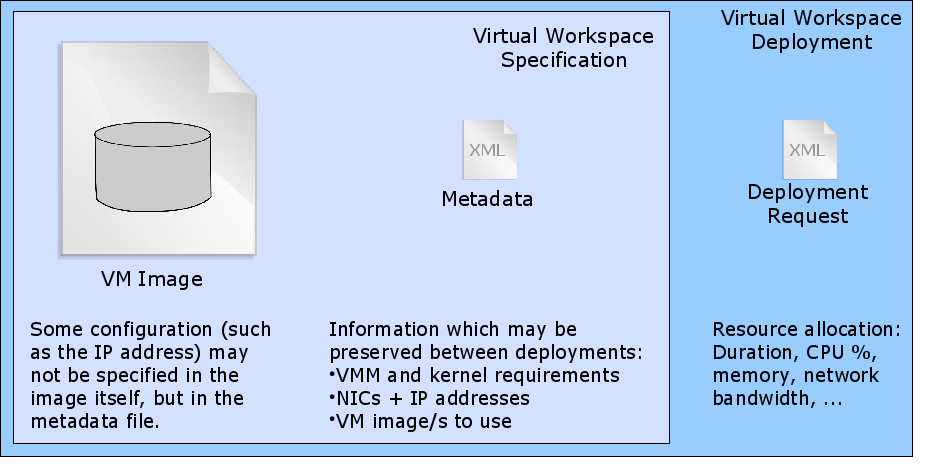
\includegraphics[width=0.85\textwidth]{figures/vw_representation.png}
    \caption{Virtual Workspace Representation}
	\label{fig:vwrepresentation}
  \end{center}
\end{figure}


A VM--based virtual workspace is composed of two elements \cite{VirtualWorkspaces05}, summarized in Figure~\ref{fig:vwrepresentation}, the \emph{VM image} and the \emph{workspace metadata}.

In a VM-based virtual workspace deployment, one or more virtual machines will be run. To instantiate a virtual machine, we need a \emph{disk image} with a runnable operating system and all the software required by the user. A VM image is composed of one or more disk images, representing the different disk partitions required by the virtual machines. Users could potentially provide their own VM images, or choose from a set of preexisting images made available by a resource provider.

Deployment--independent configuration is factored out of the VM image and into an XML \emph{metadata file}. This approach allows workspaces to be described in terms of \emph{VM image templates}, generic reusable VM images with the system software and tools for some specific purpose (e.g. a worker node for an Open Science Grid cluster), but lacking all the configuration specific to a particular type of deployment. This configuration, contained in the metadata file, is \emph{bound} to the VM image at runtime to produce an \emph{image instance}.

To better illustrate the concept of ``image templates'' and why information in the metadata file is ``deployment--independent'' we present the following example:

\begin{enumerate}
\item A user wishes to deploy a virtual workspace representing an Open Science Grid (OSG) cluster with 100 worker nodes (for the purposes of this example, we will ignore the head node and focus only on the worker nodes). We assume that worker nodes only differ in their network configuration, and that the user wants to manually specify a single private IP address for each worker node (and not rely on other mechanisms, such as DHCP). So, since each worker node will have a different network configuration, the user could prepare 100 worker node images, $W_1\ldots W_{100}$, which differ only in their network configuration. By using image templates and metadata files, the user only needs to provide a \emph{single} VM image $W$ and a metadata file $mf$ containing the network configuration of each of the worker nodes ($conf_1\ldots conf_{100}$).
\item When the virtual workspace is deployed, multiple copies of the image template are made, and each is bound to the configuration contained in the metadata file to produce runnable image instances (e.g. $W(conf_{42})=W_{42}$). So, the image template is \emph{reusable}, since a single copy of an image template can be used to yield multiple image instances.
\item In future deployments, metadata file $mf$ can be reused whenever we want to deploy a 100--node OSG cluster. In this sense, the configuration information contained in the metadata file is \emph{deployment--independent}.
\item In the future, the user wishes to deploy a 150--node cluster, using the same VM image $W$. Metadata file $mf$ cannot be used as it only includes configuration for 100 nodes. To deploy the new workspace, the user must create a new metadata file, $mf'$, with configuration for all the nodes ($conf_1\ldots conf_{150}$. Similarly, if the user wishes to deploy the 100--node cluster but using network addresses different from the ones specified in $mf$, a new metadata file would also be required in this case. Therefore, we consider that any configuration information that \emph{need not} change across deployments is deployment--independent. Furthermore, this also shows how an image template can be reused not just in a single deployment (by using it to create multiple image instances) but across deployments, since all potentially mutable information is contained in the metadata file, not in the VM image.
\end{enumerate}

In Section~\ref{cha:scheduling} we will explore optimization which result from the use of metadata files and the reusability of image templates.

Finally, when a virtual workspace is deployed, we must also specify a \emph{deployment request} (also shown in Figure~\ref{fig:vwrepresentation}). This request is an XML document describing the resource
allocation that should be assigned to the workspace, including both availability and hardware requirements (such as memory and
CPU\%). Since resource allocation requirements generally vary across deployments (e.g. in one deployment the user might be interested in performing CPU--intensive work, and I/O--intensive work in a different deployment), and also \emph{during} a deployment (to adapt to changing requirements and conditions), the deployment request includes all the \emph{deployment--dependent} parameters.


\subsection{GT4 Workspace Service}

\begin{figure}
  \begin{center}
    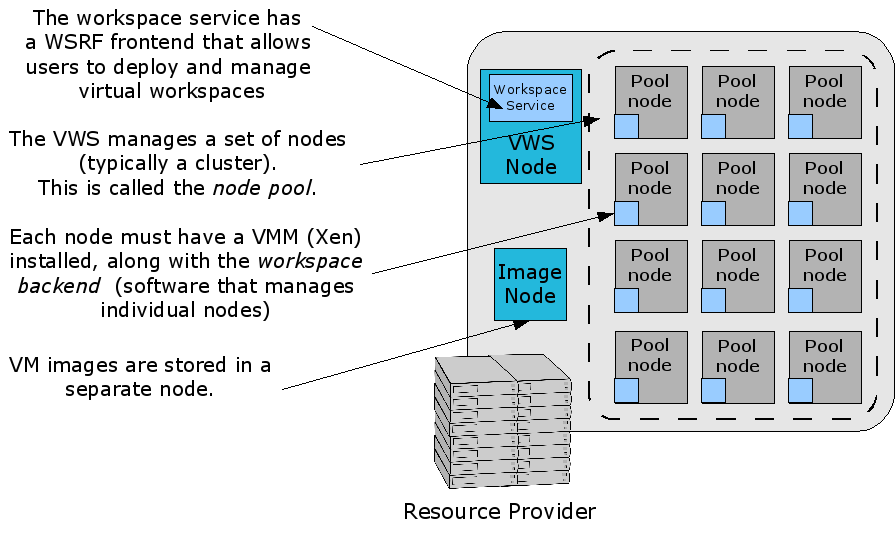
\includegraphics[width=\textwidth]{figures/vw_overview.png}
    \caption{Virtual Workspace Service}
	\label{fig:vwservice}
  \end{center}
\end{figure}


The GT4 Virtual Workspace Service \cite{vwsweb}, or VWS, which we extend in this work, allows an authorized users to request the creation of VM--based virtual workspaces through a Web Services interface. This interface also allows users to monitor and control the virtual workspace. As of this writing, the VWS only supports single--node virtual workspaces and immediate reservations without the possibility of queueing or preemption (i.e. requests for which resources cannot be immediately provisioned are rejected). Virtual machines are instantiated using the Xen Virtual Machine Monitor \cite{xen}, although others (such as VMWare \cite{vmwareweb}) could potentially be used.

Figure~\ref{fig:vwservice} shows the typical setup required by the VWS in the resource provider:

\begin{itemize}
\item A publicly accessible node, the \emph{VWS node}, hosts the Web Service frontend of the VWS.
\item A set of nodes, the \emph{node pool} are put under the control of the VWS. Virtual workspaces will be deployed on these nodes.
\item Each node in the node pool must have a virtual machine manager installed, along with the \emph{workspace backend}, a script that manages individual nodes and is invoked by the VWS when tasks need to be performed on nodes (such as starting and stopping virtual machines.
\item A separate node, the \emph{image node} acts as a repository for VM images. When a virtual workspace is deployed on the node pool, VM images are staged to the nodes from the image node.
\end{itemize}

In a typical interaction with the VWS, the following steps would take place:

\begin{enumerate}
\item A user wishes to deploy a virtual workspace. To do this, the user must provide the VM image, the workspace metadata, and the deployment request (as described in the previous section). However, the user does not need to include the potentially large VM image in the request. A reference to the location of the image in the resource provider's image node, or in a third--party site, is enough.
\item The VWS determines if there are enough resources immediately available to satisfy the request. If not, the request is rejected. Otherwise, the VWS initiates a transfer of the VM image from the image node, or a third party--site, to the nodes where that VM image will be used.
\item Once the image transfer is completed, the VWS uses the workspace backend to start the virtual machines for the requested workspace.
\item Information about the workspace, such as its status, the IP addresses assigned to the virtual machines, etc. are published through the Web Services interface (more specifically, using WSRF Resource Properties).
\item Users can query these Resource Properties, and interact with their workspaces the same way they would with a physical machine.
\item Users can also use the Web Services interface to control their workspaces (e.g. to stop them when they are done with their work)
\end{enumerate}

\chapter{Resource Management Scenarios}
\label{cha:scenarios}

Our work is motivated by a variety of use cases with quality of life and service requirements that can be met by virtual workspaces. For example:

\begin{description}
\item [Virtual labs]: A university wishes to teach a course on Parallel Programming, but lacks a cluster on which students can run their exercises, labs, etc. Even with a cluster in the university, the cluster administrator is unlikely to grant students complete control of the cluster during class hours. A virtual workspace can be dynamically created during the times when the course's labs are in session, providing students with an execution environment where they can do their exercises.
\item [Urgent computing]: Event-driven applications, such as those requiring large amounts of computational resources when an event arrives (such as data arriving from an experiment) or emergency applications, such as flood modeling, require systems that can \emph{immediately} provision resources, adequately preempting any other work taking place on the computational resources. The Special PRiority and Urgent Computing Environment \cite{spruceweb}, or SPRUCE, provides such a system, but VM--based virtual workspaces could also be used to meet the quality of service requirements of urgent computing, thanks to their ability to dynamically reshape resource allocations and seamlessly suspend and resume computations.
\item [Batch jobs with strict software requirements]: Users who need to run batch--style jobs, but require very specific software environments (e.g. legacy environments) which system administrators may not be willing to provide as they have to take into account the software needs of all their users. Virtual workspaces can provide users with exactly the software environment they need to run their jobs.
\end{description}

Our goal is to arrive at a resource management model which can meet the requirements of the above use cases. In particular, we concern ourselves here with \emph{availability}. Freeman et al. \cite{DBLP:conf/icsoc/FreemanKFRSW06} explored the protocols and enforcement methods along other resource dimensions, such as CPU and network bandwidth, highlighting the interdependencies which can arise between different resource dimensions. We leave a more exhaustive discussion of multi--dimensional resource management for future work.

Before discussing the different availability scenarios that arise in these use cases, and which will be the object or our investigations, we present the following definitions:

\begin{description}
\item[Agreement:]  We adopt the definition provided in the WS-Agreement specification~\cite{wasg}: \emph{``An agreement defines a dynamically--established and dynamically--managed relationship between parties. The object of this relationship is the delivery
of a service by one of the parties within the context of the agreement. The management of this delivery is achieved by agreeing on the respective roles, rights and obligations of the parties. The agreement may specify not only functional properties for identification or creation of the service, but also non-functional properties of the service such as performance or availability. [\ldots].''} In the context of our work, the two parties involved are a resource provider and a resource consumer (which we will refer to simply as the \emph{user}). The service to be provided is access to computational resources, and we focus on satisfying the availability requirements specified by the user.
\item[Availability:] A period defined by agreed--upon events happening at any time while the agreement is valid. During this period of time, the resources requested by the user are guaranteed to be accessible.
\item[Submission time:] Precise instant in time in which a user establishes an agreement with the resource provider. The period during which the agreement is valid need not start at the submission time (e.g., an agreement for future use of resources)
\item[Event:] An occurrence that affects availability. An event can only arrive during the time when the agreement is valid, and we currently constrain this definition to occurrences that determine the start or end of the availability. Examples of events include:
\begin{itemize}
\item \emph{User request}: The user explicitly requests the start or termination of the availability period.
\item \emph{Asynchronous events}: The user defines an asynchronous event, such as arrival of data from an experiment, that must trigger the start of the availability period (e.g., because we need computational resources to analyze the data arriving from the experiment).
\item \emph{Scheduling events}: Events emanating from a resource manager, which will determine start and end times of the availability period based on local policies, or on pre--agreed times.
\end{itemize}
\end{description}


\begin{figure}
  \begin{center}
    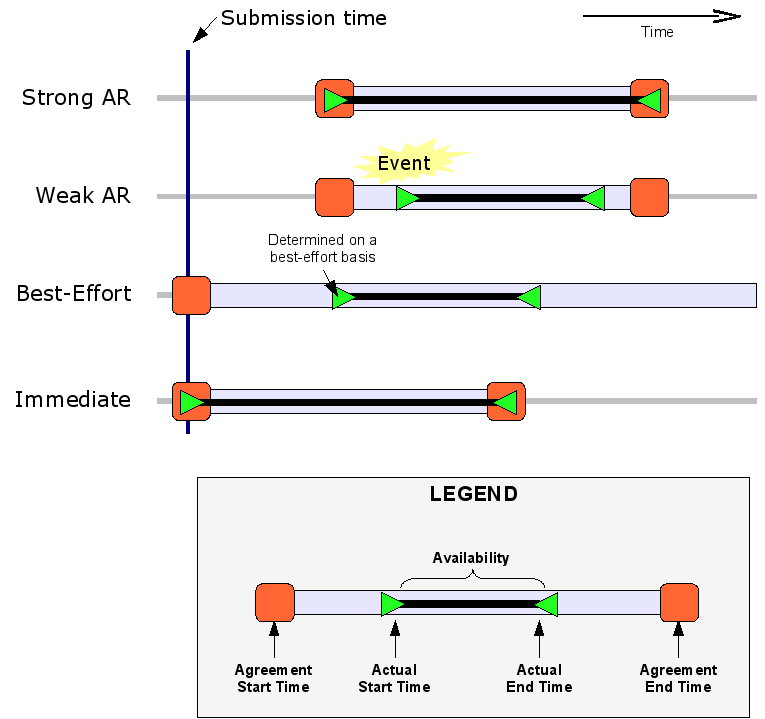
\includegraphics[width=\textwidth]{figures/availability.png}
    \caption{Availability scenarios}
    \label{fig:availability}
  \end{center}
\end{figure}

Depending on how strictly availability is defined, we encounter different \emph{availability scenarios}, which can be described with terms such as `advance reservations', `batch submissions', `best--effort scheduling', etc. Since these terms tend to be highly overloaded, throughout this text we will observe the following definitions (summarized in Figure~\ref{fig:availability}):

\begin{description}
\item[Strong Advance Reservation]: Availability in this case is clearly defined \emph{in advance} with pre--agreed a start and end timestamps, which coincide with the start and end of the agreement. Virtual workspaces for the \emph{Virtual Labs} use case, for example, will have specific start and end times (e.g. a lab which is taught from 2pm to 4pm).
\item[Weak Advance Reservation]: In event--driven applications, availability requirements are loosely defined, since the user can only specify the availability period in terms of asynchronous events (and, possibly, also a window of time during which those events are likely to arrive). However, when that event is received, availability \emph{must} be guaranteed at exactly that time, and for the duration specified. Thus, this availability scenario is an advance reservation insofar as the resource requirements are known in advance, meaning the scheduler can take steps to preemptively provision resources in case the start event arrives, but the exact start and end times are not. The Urgent Computing use case is an example of Weak AR.
\item[Best--effort Reservation]: Similarly to Weak AR, this availability scenario presents loosely defined availability requirements. However, the user agrees to have availability defined by the resource manager, which will provision resources on a best--effort basis, taking into account local policies regarding prioritization and quotas, and queueing requests if necessary. Batch jobs are an example of this availability scenario.  
\item[Immediate Reservation]: In this case, availability requirements are not known until the time the resource request arrives and, once it arrives, resources must be immediately provisioned. Unlike Weak AR, the resource manager would have no way of preemptively provisioning resources for this kind of resources, and a request is rejected if resources cannot be immediately provisioned. This scenario is, arguably, just a concrete case of Strong AR, where the interval between the resource request and the start time is zero.
\end{description}

In this paper we focus on Strong Advance Reservations\footnote{Unless otherwise noted, when we refer to an \emph{advance reservation}, or an AR, we refer to a Strong Advance Reservation}. We also touch upon Best--effort Reservations and, in particular, on how to adequately schedule workloads presenting both advance reservations and best--effort reservations.

\chapter{Modeling Virtual Resources}
\label{cha:virtualresources}

\begin{figure}
  \begin{center}
    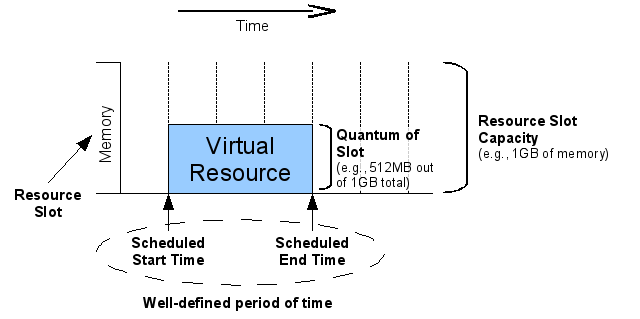
\includegraphics[width=0.8\textwidth]{figures/resourceslot.png}
    \caption{Resource Slot and Virtual Resource}
	\label{fig:resourceslot}
  \end{center}
\end{figure}

In this section, we present a resource management model which enables \emph{accurate} and \emph{efficient} creation and management of virtual workspaces in the resource management scenarios described in the previous section. Our model assumes a set of physical resources providing a set of \emph{resource slots} (e.g., all the physical memory is one resource slot, each CPU is another resource slot, etc.). A quantum of a slot (e.g., 512 MB of memory, out of the 4 GB available) may be bound to a virtual workspace to provide it with some hardware resources needed to support the workspace's activities for a \emph{well{}-defined period of time}. We term such a binding of a portion of a slot to a virtual workspace a \emph{virtual resource}. All these concepts are summarized in Figure~\ref{fig:resourceslot}

Existing local resource managers, geared towards managing the execution of jobs, are not adequate for scheduling virtual resources because they would not take into account the overhead involved in deploying and managing those virtual resources. In particular, we encounter two types of overhead: \emph{preparation overhead} and \emph{runtime overhead}. The former refers to the cost of preparing the environment where the virtual workspace will run (most notably, deploying the VM images required by that workspace), while the latter refers to the memory, CPU and I/O overhead incurred by the VM hypervisor itself. Furthermore, these overheads are not necessarily constant, and may depend on the size of the requested virtual resources, the hypervisor used, and the quality of base resources.

\begin{figure}
  \begin{center}
(a)

    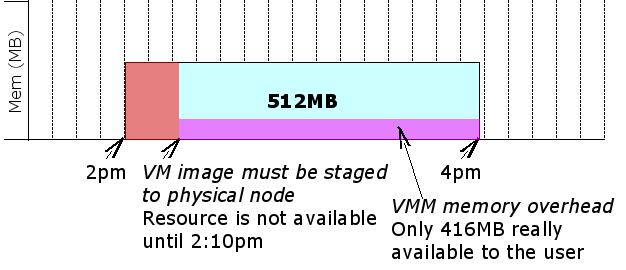
\includegraphics[width=0.8\textwidth]{figures/virtualresources_a.png}

\vspace{3em}
(b)

    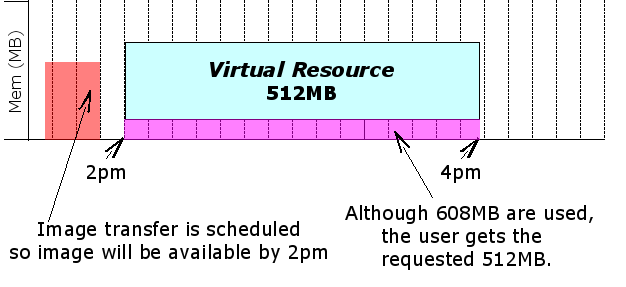
\includegraphics[width=0.8\textwidth]{figures/virtualresources_b.png}



    \caption{Virtual Resources and Overhead: (a) without considering overhead separately, and (b) considering overhead separately}
	\label{fig:virtualresources}
  \end{center}
\end{figure}

For example, let us assume that memory and time (availability) are the only two apportionable resources, and that a user requests 512MB of memory from 2pm to 4pm to support the execution of a workspace. Figure~\ref{fig:virtualresources}(a) shows how the resources allocated to the user would be invaded by two types of overhead: the preparation overhead of transferring the (potentially large) workspace's VM image to the physical node where it will run, delaying the start time of the workspace, and the runtime overhead of the virtual machine monitor. 

Using existing local resource managers, even those with AR capabilities, affects the accuracy of virtual workspace deployments, since they burden users with having to factor in the different types of overhead into their resource requests. This is not easy because users cannot accurately predict the time to stage the VM image, as they are unaware of the network traffic conditions on the site, and they have no control over how much of the virtual machine monitor's overhead will be deducted from their allocation (e.g., if several VM's are deployed on a single physical node, the deduction might be shared).

Thus, we argue in favor of a \emph{virtual resource management model}, where users get \emph{exactly} the resources they requested. To accomplish this, portions of resource slots can be bound either to virtual resources \emph{or}
to overhead in our model. The virtual resource accurately represents the resources requested by the user, and overhead is managed \emph{separately}, instead of being \emph{deducted} from the user's allocation. This results in more work for the local scheduler, which must now schedule both the virtual resource and the overhead, but results in increased accuracy and, as we will discuss in the following sections, enables the scheduler to take steps towards reducing overhead (increased efficiency).

For example, Figure~\ref{fig:virtualresources}(b) shows how a user's request for 512MB of memory from 2pm to 4pm is processed accurately by (1) \emph{scheduling} the preparation overhead of transferring the VM image (by prestaging it to the physical node before the scheduled start time of the virtual resource) and by (2) setting aside enough memory for the runtime overhead of the virtual machine without deducting it from the virtual resource.

Nonetheless, managing virtual resources and overhead involves challenges along several dimensions:

\begin{description}
\item[Time] (or \emph{availability}: We must guarantee that resources are available at the agreed--upon time, and must be able to reject requests that are deemed infeasible because it would not be possible to set up the required environment on time.
\item[Memory]: We must take into account that part of the memory in a physical node must be assigned to the virtual machine monitor. This dimension is trivial, since this memory usage is generally constant.
\item[Networking]: We must take into account that network bandwidth is shared by all the VMs on a physical node and with preparation overhead (such as image staging). Furthermore, network usage can affect CPU usage in the virtual machine monitor.
\item[Disk]: Similarly to networking, disk I/O is shared by all VMs on a node and can affect CPU usage in the virtual machine monitor. Furthermore, physical nodes must have enough disk space to support the VM images of different workspaces
\item[CPU]: The CPU share required by the virtual machine monitor can vary over time, depending on the resource usage of the VMs it is managing.
\end{description}

As mentioned in the introduction, we concern ourselves here with the resource dimension of availability, which is primarily impacted by preparation overhead. In particular, workspace deployment can involve the (potentially expensive) transfer of a VM image to a node, a task that requires I/O and network usage that has to be accounted for by the scheduler. However, we currently assume that VMs produce no network activity that would share bandwidth with preparation overhead (i.e. the Networking dimension does not affect the Time dimension).

The management of runtime overhead for the Xen virtual machine monitor was already explored by Freeman et al. \cite{DBLP:conf/icsoc/FreemanKFRSW06}, and we leave an investigation of multi--dimensional scheduling of both preparation and runtime overhead for future work.


\chapter{VW Scheduler Prototype}
\label{cha:scheduling}

In this section we describe how we extend the Workspace Service to support the AR and ASAP scenarios described in Section~\ref{cha:scenarios}. We do this by creating a scheduler prototype which schedules virtual resources and preparation overhead separately, using scheduling strategies designed to increase accuracy and efficiency.

\section{Service Interface}

We extend the Workspace Service interface to allow the user to specify the time constraints of the virtual resources required by a VW. Specifically, we extend the deployment request document (see Section~\ref{sec:vwrepresentation}) to include the start time and end time of the virtual resource(s) to be allocated to the workspace. These times can be expressed as exact timestamps, as a time interval within which an asynchronous event can be received (triggering the start or end of the workspace), or omitted (in which case the workspace must be scheduled as soon as possible).

\section{Design}

We propose two enhancements to existing local resource managers that enable them to schedule preparation overhead separately in a manner consistent with our model: deadline--driven \emph{file staging strategies} that budget enough resources to accommodate the overhead of transferring VM images, and \emph{VM image caches} to reduce the number of image transfers performed.

\subsection{File staging strategies}
\label{sec:filestaging}

\begin{figure}
  \begin{center}
    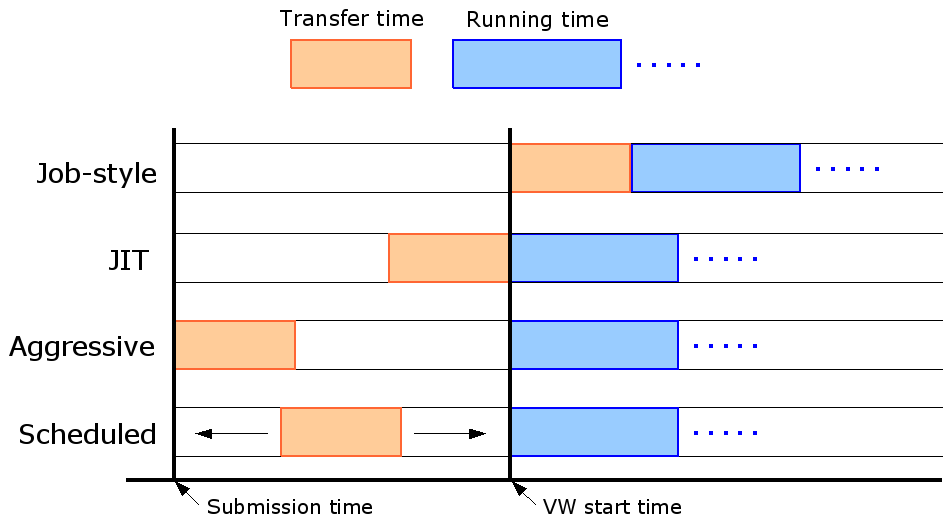
\includegraphics[width=0.8\textwidth]{figures/filetransfer.png}
    \caption{File Staging Strategies}
	\label{fig:filetransfer}
  \end{center}
\end{figure}

Jobs submitted to batch schedulers generally assume that required files are available in the worker nodes (e.g., through an NFS drive) or that the input files will be staged to the worker nodes when the job starts. As discussed in the previous section, this assumption presents problems for deploying time{}-sensitive VWs, as VM images can be large and costly to transfer, and transfer times can consume a significant portion of the time allocated to the user. Thus, even if a resource is made available at a requested time $t$, it may not be ready for use until a significantly later time $t+d$.

These problems can be solved in some cases by providing the scheduler with application--specific information about what data needs to be transferred for each deployment, enabling it to distinguish cases where prestaging the data before the scheduled start time $t$ would be appropriate. In particular, in the case of a virtual workspace, the scheduler should use a \emph{Scheduled} file transfer strategy: after estimating the amount of preparation overhead (the time necessary to transfer all required VM images), the image transfers are scheduled in such a way that they will be completely deployed by time $t$. The scheduler will reject workspaces where such an image transfer cannot be scheduled (even if all other resources, such as CPU and memory, are available during the requested period of time). 

The application--specific information provided to the scheduler not only allows it to distinguish what file staging strategy would be appropriate at each point, but also allows it to correctly estimate the preparation overhead. To do this, the application--specific information provided to the scheduler is the workspace metadata file (see Section~\ref{sec:vwrepresentation}). In particular, the overhead estimate can be computed based on (1) an image descriptor (currently the location of the image file within an image repository node), (2) image size, and (3) number of nodes in the VW to estimate what the preparation overhead will be.

Of course, it could be argued that simply adding basic improvements to \emph{``Job--style''} file staging (where the data is staged at the beginning of a job's resource allocation) could already result in improved accuracy, without going to the extreme of scheduling the preparation overhead separately. To that effect, we also consider the following na\"ive file strategies to compare their performance to the \emph{Scheduled} approach. 

\begin{description}
\item[Just In Time (JIT)]. Assuming the network's full bandwidth is available for staging the necessary VM image for a workspace, the scheduler estimates the time required to transfer the image and starts the transfer before the start time, allocating just enough time to transfer the image.
\item[Aggressive]: This strategy attempts to transfer images immediately after the request has been accepted, regardless of the
starting time for the image transfer.
\end{description}

Note that these two strategies (along with \emph{Job--Style}) are not scheduled approaches to file staging since the file transfer start time depends uniquely on either the starting time of the workspace (\emph{JIT}) or the submission time (\emph{Aggressive}), without consideration for other submissions or resource usage. Figure~\ref{fig:filetransfer} summarizes all these file staging strategies.

\subsection{Image caches}
\label{sec:imagecaches}
Adequate VM image staging affects \emph{accuracy}, by making sure that all preparation overhead is processed before the virtual workspace's scheduled start time. We also wish to improve \emph{efficiency} by reducing preparation overhead whenever possible. We can accomplish this through the use of \emph{VM image template caches} (or simply \emph{image caches}). As described in Section~\ref{sec:vwrepresentation}, factoring deployment--independent configuration information out of the VM image and into a metadata file allows VM images to be reusable. In particular, a VM image can be deployed to a physical machine, and used multiple times by making local copies and binding those copies to potentially different metadata files. This reusability enables us to cache image templates on physical node, thus reducing the number of image transfer.

The image cache keeps a copy of a subset of all available template images according to a caching strategy (we currently support LFU and LRU, with a configurable cache size). When an image has to be deployed to a physical node, the scheduler favors nodes that already have a cached copy of the required image template. Because caches enable some images to be instantly available in
the nodes, they benefit both AR deployments, since it will be possible to accept starting times that would ordinarily be unfeasible if the image first had to be transferred to the nodes, and ASAP deployments, by allowing workspaces to start running sooner. Additionally, our image caches are implemented to avoid redundant transfers when deploying a new image template to a node, as for example when the same image template is required to produce two image instances on a node, in which case the template is transferred only once.

\section{Implementation}

To implement these enhancements, we add a layer of scripts on top of an existing local resource manager, Sun Grid Engine
\cite{sgeweb}, or SGE. These scripts take the application--specific information of virtual workspaces (the metadata file), and use SGE to schedule not only the virtual resources, but also the preparation overhead. Additionally, SGE is made aware of the state of image caches in the physical nodes, so it will take them into account in its scheduling decisions.

SGE was chosen because it is an easily extensible local resource manager, facilitating the task of implementing our enhancements on top of it. Nonetheless, other local resource managers could potentially be used, although our goal is to eventually arrive at a resource manager that incorporates our virtual resource management model in the scheduler component itself, and not as a layer on top of it\footnote{As of this draft, a more elaborate implementation, including an external Advance Reservation server to schedule advance reservations, which are not natively supported by SGE. More details will be included in the final draft of this paper.}.


\chapter{Experiments}
\label{cha:experiments}
We present a series of experiments that illustrate the effect of using
the scheduling model and techniques discussed in the previous section.
These experiments focus on evaluating our techniques for managing the
overhead of transferring VM images to the nodes where they are
deployed.

Our experiments were run on a testbed composed of 10 dual{}-CPU Pentium
III 500 MHz systems, each with 512 MB of RAM and 9G of local disk. One
node was used as a cluster head node, eight nodes for VM deployment,
and the remaining node as an image repository node, from which the VM
images would be transferred to the worker nodes. Nodes were connected
using 100 Mb/s switched Ethernet.

Virtual machine images were deployed using the SGE scheduler with the
extensions described above, based on traces that we developed for both
the advance reservation (AR) and batch (ASAP) cases. For the ASAP
cases, we used real workload traces, while for the AR cases, lacking
real AR submission workloads, we produced artificial traces using a
trace generator.


For all our experiments, we assumed that all virtual workspace requests
involved the same amount of CPU\% and memory for each virtual node. We
allowed at most 2 VMs to be deployed to a single physical node. Since
we focus on preparation overhead, the VW remains idle during its
runtime, and we assume that the VM generates no network traffic that
would share bandwidth with preparation overhead. This assumption is
reasonable in the case of highly parallel applications.

\section{Scheduling Jobs versus Scheduling VMs}

Our first set of experiments investigates to what extent using
information on the relatively manageable overhead of VM scheduling can
improve the accuracy of providing a virtual resource to a
deadline{}-sensitive client. We assume that the client requests the
resource for a fixed time interval and we calculate accuracy (or
``client satisfaction'') as the ratio of the time the client actually
got to the requested time. Lacking any AR traces or AR trace generator,
we developed a simple trace generator capable of generating a large
number of requests according to a set of parameters. We then ran an
offline admission control algorithm (derived from Earliest{}-Deadline
First \cite{BorjaCite22}) on those requests to ensure that there exists a feasible
schedule for the submissions in the trace. Each submission represents
the deployment of a virtual cluster configured with the software
required to applications commonly run on the Open Science Grid (OSG),
and includes (1) the descriptor of the image template to use, (2) the
number of nodes, (3) the starting time of the workspace, and (4) its
duration. The Xen VM image with OSG worker node support that we used in
this experiment is 600 MB in size \cite{DBLP:conf/ccgrid/FosterFKSSZ06}.


\newcolumntype{M}{>{\centering}m{0.15\textwidth}}
\newcolumntype{N}{>{\centering}m{0.3\textwidth}}

\begin{table}
\begin{center}
\begin{tabular}{|M|MM|MM|}

\cline{2-5}
\multicolumn{1}{M|}{}&
\multicolumn{1}{M|}{\bfseries Trace I}&
\multicolumn{1}{M|}{\bfseries Trace II}&
\multicolumn{1}{M|}{\bfseries Trace III}&
\multicolumn{1}{M|}{\bfseries Trace IV}

\\\hline

{\bfseries Trace duration (s)} &
\multicolumn{2}{N|}{7200}&
\multicolumn{2}{N|}{4700}

\\\hline

{\centering\bfseries \#~VW \nohyphens{submissions}} &
\multicolumn{1}{M|}{36}&
35 &
\multicolumn{2}{N|}{62}

\\\hline

{\bfseries Nodes per VW} &
\multicolumn{2}{N|}{2{}-4\newline (Uniformly distributed)} &
\multicolumn{2}{N|}{2{}-16\newline (Derived from original trace)}

\\\hline

{\bfseries Total images to deploy} &
\multicolumn{1}{M|}{110 (66.0GB)} &
{106\newline (63.6GB) } &
\multicolumn{2}{N|}{114 (86.4GB)}

\\\hline

{\bfseries VW Duration} &
\multicolumn{2}{N|}{1800s} &
\multicolumn{2}{N|}{Avg=53.0s\newline StDev=4.24s}

\\\hline

{\bfseries Starting times} &
\multicolumn{1}{M|}{Uniformly Distributed} &
{Clustered in 100s windows every 900s} &
\multicolumn{2}{N|}{\centering ASAP}

\\\hline

{\bfseries Images used} &
\multicolumn{2}{N|}{6 600MB images,\newline uniformly distributed} &
\multicolumn{2}{N|}{See Table 2}

\\\hline
\end{tabular}

\caption{Traces used in experiments}
\label{tab:traces}
\end{center}
\end{table}

Table~\ref{tab:traces} describes the two traces (I and II) used in this experiment.
These two traces differ in how the starting times of the VWs are
distributed throughout the duration of the experiment. In Trace I, the
starting times are distributed uniformly throughout the trace, while in
Trace II the starting times appear only during 100s windows (each
occurring every 900s), simulating VWs that are submitted in a bursty
fashion.

\begin{figure}
  \begin{center}
    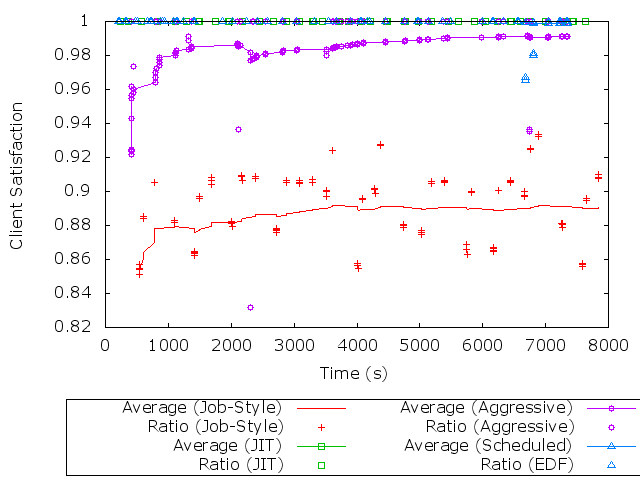
\includegraphics[width=0.8\textwidth]{figures/ClientSatisfaction-UniformStartTimes.png}
    \caption{Client Satisfaction (Trace I)}
	\label{fig:clientsatisfactionI}
  \end{center}
\end{figure}

Figure~\ref{fig:clientsatisfactionI} shows the results of running Trace I with the scheduling
strategies described in Section~\ref{sec:filestaging} (\emph{JIT, Aggressive, and
Scheduled}) and pits them against the baseline unmodified SGE
(\emph{Job{}-Style)} that does not seek to prestage VM images but
instead stages required files during the availability of the physical
resources. We see that \emph{Scheduled} and \emph{JIT} achieve 100\%
client satisfaction in most cases, followed by \emph{Aggressive }with
most submissions in the 96\%{}-100\% range. Since this trace represents
a best{}-case scenario, where the start times are uniformly distributed
throughout the experiment, even the na\"ive \emph{JIT} and
\emph{Aggressive} strategies achieve good performance.

\begin{figure}
  \begin{center}
    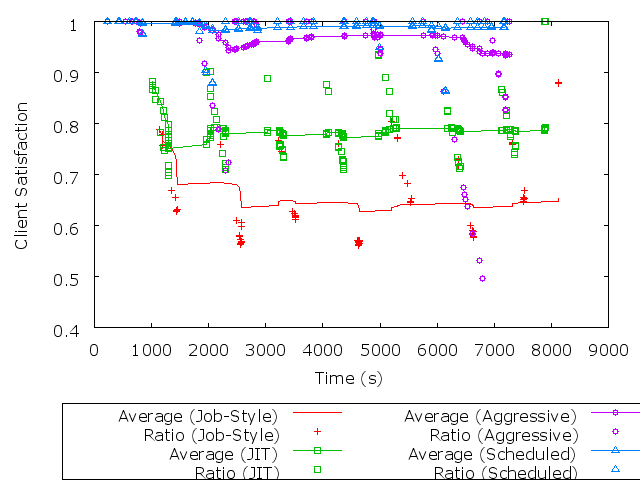
\includegraphics[width=0.8\textwidth]{figures/ClientSatisfaction-ClusteredStartTimes.png}
    \caption{Client Satisfaction (Trace II)}
	\label{fig:clientsatisfactionII}
  \end{center}
\end{figure}

Figure~\ref{fig:clientsatisfactionII} shows results with Trace II. Since \emph{JIT} allows just
enough time to transfer the image, regardless of what other VWs are
scheduled, this strategy can result in multiple image transfers being
scheduled during the same period of time (right before the ``window'').
As those transfers share available bandwidth, they take longer than
estimated. \emph{Scheduled} addressed this problem by prioritizing image
transfers and making use of network idle time, resulting in the best
performance, with few non{}-100\% satisfaction instances (and always at
the end of a ``window''). \emph{Aggressive}, on average, also has
good performance, but the images with tighter deadlines suffer as the
result of having to share bandwidth with other transfers.

\emph{Scheduled} is the only approach that
actually schedules a resource slot for the preparation overhead with
the goal of maximizing client satisfaction, while the other strategies
na\"ively start the image transfers at fixed times. By scheduling
overhead in the same way as virtual resources, instead of assuming that
overhead should be absorbed into the client's requested virtual
resource, \emph{Hybrid} achieves the best client satisfaction in the
two submission patterns present in traces I and II.

\section{Optimizing Image Transfer}

Our second set of experiments investigate two things: (1) how much in
terms of bandwidth usage the resource provider can save through
judicious use of image caching based on workspace metadata and (2) to
what extent image caching can improve deployment time (and thus also
client satisfaction) in situations where VM availability is requested
to start ASAP. 

Since this experiment focuses on ASAP submissions, the same type of
submissions commonly found in batch systems, we were able to use a real
workload. In particular, we used the San Diego Supercomputer Center
(SDSC) DataStar log, available at the Parallel Workloads Archive \cite{BorjaCite21}.
We chose this workload because it explicitly distinguished submissions
for the DataStar's express queue (eight 8{}-CPU nodes, accepting jobs
lasting at most 2 hr), which allows us to test a scenario in which
minimizing deployment overhead is specially important: short{}-lasting
jobs. Since the SDSC DataStar log spans several months, we selected an
80 minute stretch of submissions (submissions \#21543 to \#21665 on
queue \#1) which we could run on our testbed. This extract was selected
because it represented a flurry of short{}-lasting jobs, which would
allow us to test how our system copes with the bandwidth requirements
of deploying a large amount of VM images.


\begin{table}
\begin{center}
\begin{tabular}{|c|c|c|c|c|}
\cline{2-5}
\multicolumn{1}{c|}{} &
\multicolumn{2}{c|}{\bfseries Trace III} &
\multicolumn{2}{c|}{\bfseries Trace IV}

\\\cline{2-5}

\multicolumn{1}{c|}{}  & {\bfseries Submissions} & {\bfseries Images} & {\bfseries Submissions} & {\bfseries Images} 

\\\hline

{\bfseries img.1} & 23\% & 21\% & 55\% & 60\%

\\\hline

{\bfseries img.2}
&
18\%
&
15\%
&
27\%
&
25\%

\\\hline

{\bfseries img.3}

&
15\%
&
12\%
&
6\%
&
6\%

\\\hline

{\bfseries img.4}
&
18\% 
&
15\%
&
5\%
&
4\%

\\\hline

{\bfseries img.5}
&
24\%
&
14\%
&
3\%
&
3\%

\\\hline

{\bfseries img.6}
&
3\%
&
12\%
&
3\%
&
3\%

\\\hline
\end{tabular}

\caption{Distribution of images in traces III, IV}
\label{tab:imagedistro}
\end{center}
\end{table}

When adapting the trace to our own experiments, each submission was
converted to a virtual cluster submission in which the number of nodes
was the number of requested processors in the original trace, scaled
down by four (the express queue has 64 processors; our testbed has 16),
with submission times and VW duration left unaltered. Each submission
was furnished with one of six 600 MB images. Two traces where produced,
with the only difference being the distribution of images assigned to
each submission. The first trace (Trace III) has images uniformly
distributed amongst the submissions, while in the second trace (Trace
IV) two images account for more than 80\% of the submissions. The
characteristics of theses traces are summarized in Table 1, while the
distribution of images is shown in Table~\ref{tab:imagedistro}. The rate at which VWs are
submitted is shown in Figure~\ref{fig:providershape}.

\begin{figure}
  \begin{center}
    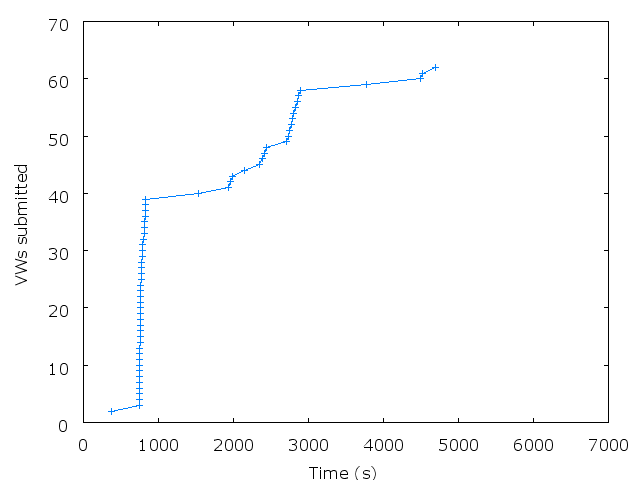
\includegraphics[width=0.8\textwidth]{figures/ProviderPerspective-TraceShape.png}
    \caption{VW Submissions (Traces III and IV)}
	\label{fig:providershape}
  \end{center}
\end{figure}

\begin{figure}
  \begin{center}
    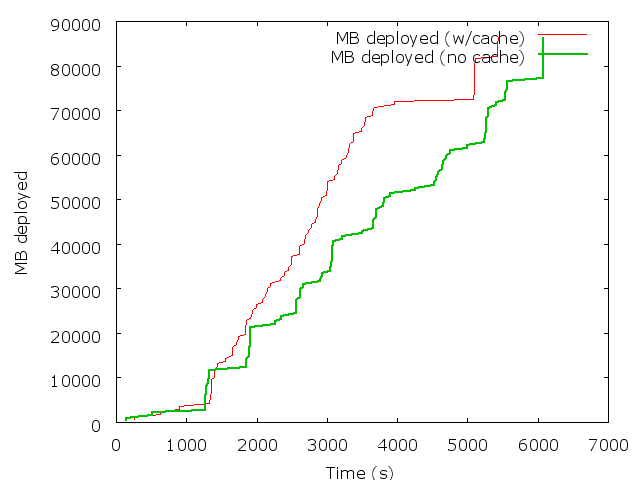
\includegraphics[width=0.8\textwidth]{figures/ProviderPerspective-Uniform2.png}
    \caption{MB Deployed (Trace III)}
	\label{fig:providerIII}
  \end{center}
\end{figure}

\begin{figure}
  \begin{center}
    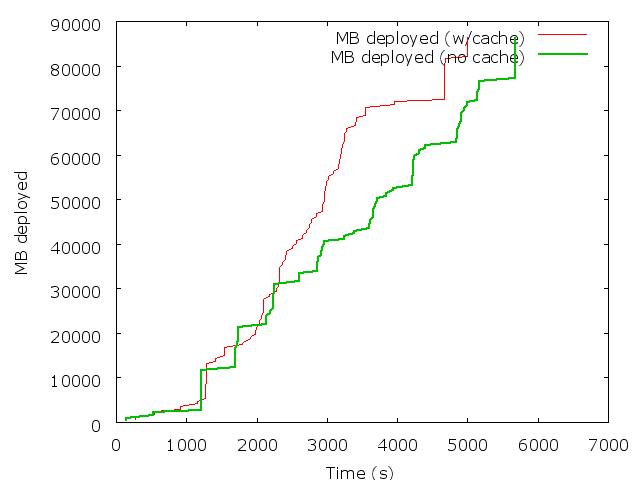
\includegraphics[width=0.8\textwidth]{figures/ProviderPerspective-Pareto2.png}
    \caption{MB Deployed (Trace IV)}
	\label{fig:providerIV}
  \end{center}
\end{figure}

To minimize deployment time and increase throughput, we used a 1.8 GB
LFU cache in each node (enough to cache three images). Figure~\ref{fig:providerIII} shows
the cumulative number of MB transferred, overlaid with the VW
submissions. We can observe how, after the 2000s mark, the rate at
which images are deployed starts to increase, thanks to the reduced
transfer time resulting from the use of a cache. The difference in
effectively deployed MB is greatest at the 3550s mark, where the cached
approach results in a 25.2 GB ``advantage'' over the non{}-cached
approach. Figure~\ref{fig:providerIV}, shows the same data from running trace IV, where
the distribution of images favors a much larger number of cache hits.
Throughput is slightly better, with a difference of 27.6 GB at that
same 3550s mark.

Deployment time (not shown in graphs) is also improved. The average
deployment time for a single image, when not using a cache, is 440s for
both traces. This time is reduced to 305s and 247s, in Trace III and IV
respectively, when using an image cache.

These two experiments highlight how using the VW metadata to cache image
templates and avoid redundant transfers benefits both the provider, by
offering a better utilization of resources leading to higher
throughput, and the consumer, by reducing the deployment time of ASAP
workspaces.


\section{Effect of cache size}

When submitting workspaces set to begin ASAP, preparation overhead may
prevent short{}-duration workspaces from being cost{}-effective. Our
final experiment explores the impact of cache size on the costs
associated with short{}-duration workspaces. Although these results are
not exhaustive, they nonetheless allow us to extract some useful
information regarding the use of image caches.

For this experiment we used two artificial stress traces in which a
series of VWs, of size one to six nodes each, were submitted at random
intervals (between 5s and 30s) for 20 minutes. Given the limited disk
space in our testbed machines, and to allow for a configuration where
all possible images could be cached in a node, we used eight 256 MB
images. In the first trace, 257 images had to be deployed, with images
being selected according to a uniform distribution. In the second
trace, 235 images had to be deployed, and two of the images accounted
for 77\% of all submissions.

\begin{table}
\begin{center}
\begin{tabular}{|>{\centering}m{0.1\textwidth}|>{\centering}m{0.07\textwidth}|c|c|c|c||>{\centering}m{0.07\textwidth}|c|c|c|c|}
\cline{2-11}
\multicolumn{1}{c|}{} &
\multicolumn{5}{c||}{\bfseries Stress Trace I} &
\multicolumn{5}{c|}{\bfseries Stress Trace II}

\\\cline{2-11}

\multicolumn{1}{c|}{}  & 
{\bfseries No cache} & {\bfseries 25\%} & {\bfseries 50\%} & {\bfseries 75\%} & {\bfseries 100\%} &
{\bfseries No cache} & {\bfseries 25\%} & {\bfseries 50\%} & {\bfseries 75\%} & {\bfseries 100\%}
\\\hline

{\bfseries Cache hits} & --- & 48 & 123 & 150 & 165 & --- & 144 & 169 & 167 & 159 

\\\hline

{\bfseries Cache misses} & --- & 126 & 80 & 60 & 54 & --- & 59 & 36 & 39 & 42

\\\hline

{\bfseries Avg. image deploy time} & 141s & 163s & 103s & 96s & 94s & 124s & 89s & 80s & 81s & 86s

\\\hline
\end{tabular}

\caption{Effect of Cache Size}
\label{tab:cache}
\end{center}
\end{table}

Table~\ref{tab:cache} shows the result of running these two traces both without a
cache and with a cache capable of holding 25\%, 50\%, 75\%, or 100\% of
the images. Note that, when a redundant transfer is avoided (as
described in Section \ref{sec:imagecaches}) it is not counted as a hit or a miss.

We see that the first trace produces similar results when using a 50\%,
75\%, or 100\% cache, but the 25\% configuration is \emph{worse} than
not using a cache at all, due to the large number of cache misses (a
cache miss results in both a download of the image \emph{and}
performing a local copy of the image). In the second trace, on the
other hand, all cache sizes produce similar results, since the 25\%
cache is already capable of holding the two most used images.

To make short{}-duration cost{}-effective, caches can help to reduce the
deployment time of images, but this time will still be bound by the
time of making a local copy in the case of a cache hit. In this
experiment, the average time to do a local copy is 60s. By precaching
images typically used for short{}-term deployments, locking them in the
image caches, and optimizing the local copy time, the
cost{}-effectiveness of short{}-duration VWs can be improved.

\chapter{Related Work}
\label{cha:related}

Many projects tackle the problem of dynamically overlaying virtual
resources on top of physical resources by using virtualization
technologies, and do so with different resource models. These models
generally consider overhead as part of the virtual resource allocated
to the user, or do not manage or attempt to reduce it. A common
assumption in related projects is that all necessary images are already
deployed on the worker nodes. Our requirements for dynamic deployment
of AR and ASAP workspaces make it impossible to make this assumption.

The Shirako system \cite{BorjaCite12} developed within the Cluster{}-On{}-Demand
project \cite{BorjaCite10, codweb} uses VMs to partition a physical cluster into several
virtual clusters. Their interfaces focus on granting \emph{leases} on
resources to users, which can be redeemed at some point in the future.
However since their model focuses on batch cases the adopted overhead
management model is to absorb it into resources used for VM deployment
and management. As we have shown, this model is not sufficient for
AR{}-style cases.

The VIOLIN and VioCluster projects \cite{BorjaCite13, viocluster, DBLP:journals/computer/RuthJXG05} allow users to overlay a
virtual cluster over more than one physical cluster, leveraging VM live
migration to perform load balancing between the different clusters. The
VioCluster model assumes that VM images are already deployed on
potential hosts, and only a ``binary diff'' file (implemented as a
small Copy{}-On{}-Write file), expressing the particular configuration
of each instance, is transferred at deploy{}-time. This is less
flexible than using image metadata, as COWs can be invalidated by
changes in the VM images. Furthermore, our work focuses on use cases
where multiple image templates might be used in a physical cluster,
which makes it impractical to prestage all the templates on all the
nodes.

The Maestro{}-VC system \cite{BorjaCite18} also explores the benefits of providing a
scheduler with application{}-specific information that can optimize its
decisions and, in fact, also leverages caches to reduce image
transfers. However, Maestro{}-VC focuses on clusters with long
lifetimes, and their model does not schedule image transfer overhead in
a deadline{}-sensitive manner, and just assumes that any image staging
overhead will be acceptable given the duration of the virtual cluster.
Our work includes short{}-lived workspaces as a case that must perform
efficiently under our model.

The Virtuoso Project \cite{BorjaCite19} and, in particular, its VSched component \cite{BorjaCite17},
is capable of co{}-scheduling both interactive and batch workloads on
individual machines in a deadline{}-sensitive manner, but does not
factor in the overhead of deploying the VMs to the nodes where they are
needed.

The In{}-VIGO project \cite{BorjaCite16} proposes adding three layers of
virtualization over grid resources to enable the creation of virtual
grids. Our work, which relates to their first layer (creating virtual
resources over physical resources), is concerned with finer{}-grained
allocations and enforcements than in the In{}-VIGO project. Although some exploration of cache-based deployment has also been done with VMPlant \cite{BorjaCite20}, this project focuses on batch as opposed to deadline-sensitive cases.

\chapter{Conclusions and Future Work}
\label{cha:conclusions}

We described a virtual resource model, and a set of scheduling
strategies for that model, based on scenarios that, in our experience,
frequently arise in the Grid. These scenarios combine batch job
platforms as well as platforms whose deployment is
deadline{}-sensitive, such as interactive platforms. VM deployment and
management overhead can be both large and highly variable, factors that
conflict with the deadline{}-sensitive availability needs of
interactive and time{}-critical platforms. Thus, our proposed model
separates resource use devoted to the overhead of VM deployment from
resources available to the VM itself, enabling us to schedule overhead
resource slots equally with VM slots.

Our results show that by modifying a scheduler to schedule workspace
preparation overhead, rather than leaving workspace preparation to the
user, we can achieve significantly better adherence to requested
availability times. (One may argue that the user could simply request
start times sooner than required, to allow time for image staging, but
this in effect corresponds to the JIT scenario, which we show is not
always effective.) Providing the scheduler with information about the
VM images needed by a virtual workspace can have two benefits. First,
the required transfer operations can be scheduled in advance. Second,
we can use information about a VM image as defined in the workspace
metadata to optimize the resource usage devoted to VM deployment by
caching the bulk of the data associated with frequently used images.
Both strategies have benefits for the resource provider and for the
client in the case of heavy load and/or immediate reservations.
Further, by reducing preparation overhead, these strategies also make
the deployment of short{}-lived VMs more cost{}-effective.

Interesting challenges arise when one considers that the network
bandwidth has to be shared not only with other VM image transfers but
also with virtual resources allocated to applications. Our further work
on this subject will involve developing models that will accommodate
such sharing, as well as managing other resource overhead arising in
the hypervisor context.

%\appendix
%\chapter{First appendix}
%\label{app:1}

% ---- Chicago Thesis Style ---- %
\newpage
\addcontentsline{toc}{chapter}{References}
\begin{singlespace}
\bibliography{masterspaper}
\bibliographystyle{abbrvurl}
\end{singlespace}

% Figures and tables, if you decide to leave them to the end
%\input{figure}
%\input{table}

\end{document}
